\documentclass{beamer}  % Use Beamer class
\usepackage{graphicx}   % Allows including images
\usepackage{wrapfig}  
\usepackage{bookmark} 

\usetheme{Madrid}       % Choose a Beamer theme (e.g., Madrid, Berlin, Warsaw, etc.)

\title{MiS Presentation}
\author{Tom Mann}
\date{\today}

\begin{document}

% Title slide
\begin{frame}
    \titlepage
\end{frame}

% Content slide
\begin{frame}{Contents}
    \begin{itemize}
        \item Context
        \item Aims
        \item Format \& Content
        \item Session 1: Introduction
        \item Session 2: M\"{o}bius Strips
        \item Session 3-4: Statistcs
        \item Session 5: Coordinate Grid
        \item Session 6: 1-2 Nim
        \item Evaluation
    \end{itemize}
\end{frame}

% Context of school
\begin{frame}{Context}
    \begin{itemize}
        \item This projcect was conducted in partnership with Our Lady and St Thomas catholic school (OLST)
        \item OLST is a co-educational primary academy located in Willington for students aged 4 - 11
        \item OLST is a small school with only on class of 18-20 students per year
        \item Project was conducted with the year 6 class
    \end{itemize}
\end{frame}

% Aims of the project, and the rational behind them
\begin{frame}{Initial consultation with school}
    \begin{itemize}
        \item Increase confidence in girls ability in maths
        \item This goes hand in hand with decreasing maths anxiey in girls
        \item In the long term this could posisbly increase performance in girls, increasing number of girls achieving 'Greater Depth' in SATs
    \end{itemize}
\end{frame}

\begin{frame}{Aims}
    \begin{itemize}
        \item Increasing confidence
        \begin{itemize}
            \item[-] Belief in their own abilities
            \item[-]Nationally girls peform at a very similar level to boys in SATs (Gov.uk, 2024)
            \item[-] Boys tend to believe more than girls do that their intellectual abilities cause their high marks in maths (Georgiou, S. N. et al, 2007)
        \end{itemize}
        \item Decreasing anxiety
        \begin{itemize}
            \item[-] Maths anxiety: feelings of nervousness or apprehension in response to a current or future  situation involving maths 
            \item[-]Women are more than twice as likely to experience maths anxiety than men (National Numeracy, 2024) 
        \end{itemize}
    \end{itemize}
\end{frame}


% Format of the project
\begin{frame}{Format \& Content}
    \begin{itemize}
        \item Lunch time sessions about 30 minutes long
        \item Only girls in the session
        \begin{itemize}
            \item[-] Girls are said to be more confident and more likely to express themselves in a single sex environment
            \item[-] Girls reported that they felt more comfortable and liked science and mathematics more
            in a single-sex setting (Baker, 2002)
        \end{itemize}
        \item The content of the sessions is not defined by the aims.
    \end{itemize}
\end{frame}

% Mathematical Content

% Logistics of sessions
% \begin{frame}{Logistics}
%     \begin{itemize}
%         \item 
%     \end{itemize}
% \end{frame}

% Slide for various sessions
% Include logistics, materials and communication
% And account of delivery including any adaptations
\begin{frame}{Session 1: Introduction}
    The aim of this project is very individual, so it is important to get to know the students I am working with.
    \begin{itemize}
        \item What is the level of maths anxiety among the girls?
        \begin{itemize}
            \item[-]Majority of girls reported some symptoms of maths anxiety
        \end{itemize}
        \item What are the causes  of maths anxiety?
        \begin{itemize}
            \item[-] Judgement
            \item[-] Fear of being left behind
            \item[-] Frustration
        \end{itemize}
        \item How can these causes be treated?
    \end{itemize}
\end{frame}

\begin{frame}{Session 2: M\"{o}bius Strips}

    \begin{columns}
        \column{0.6\textwidth}
        \begin{itemize}
            \item Design:
            \begin{itemize}
                \item[-] No numbers
                \item[-] Focus on the process rather than the outcome
                \item[-] Intrinsic value intervention
            \end{itemize} 
            \item This session involved the girls constructing and exploring the physical properties of a M\"{o}bius strip
            \item The aim of this session was to allow the girs to enjoy the process of exploring new ideas 
            
        \end{itemize}
        \column{0.4\textwidth}
        \begin{figure}
            \includegraphics[scale = 0.2]{Images/Möbius_Strip.jpg}
            \caption{M\"{o}bius Strip}
        \end{figure}
    \end{columns}
\end{frame}

\begin{frame}{Session 2: M\"{o}bius Strips}
    \begin{itemize}
        \item The session consisted of 3 main activities
        \begin{enumerate}
            \item Creating the M\"{o}bius strips
            \item Drawing on the M\"{o}bius strips
            \item Cutting the  M\"{o}bius strups
        \end{enumerate}

        \vspace{10pt}

        \item Evaluation
        \begin{itemize}
            \item[-] The session defnitely promoted curiosity and creativity  (maybe a bit too much)
            \item[-] The students enjoyed working through not understanding something 
            \item[-] Some of the activites were too fiddly 
        \end{itemize}
    \end{itemize}
\end{frame}
\begin{frame}{Session 3: Statistics - Data collection}
    \begin{columns}
        \column{0.55\textwidth}
            \begin{itemize}
                \item Design:
                \begin{itemize}
                    \item[-] Utility value intervention
                    \item[-] Getting comfortable disussing maths
                \end{itemize}
            \end{itemize}
            \begin{enumerate}
                \item What is statistics?
                \begin{itemize}
                    \item[-] How do we collect data?
                    \item[-] How do we analyse data?
                    \item[-] Why is statistics useful?
                \end{itemize}
                \item Students collecting their own data         
                \item Talking about maths at home
            \end{enumerate}
        \column{0.45\textwidth}
            \begin{figure}
                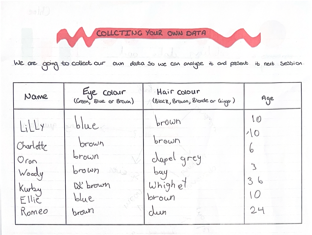
\includegraphics[scale = 0.49]{Images/Collecting_data_example.png}
                \caption{Example of data a student collected}
            \end{figure}
    \end{columns}
        
\end{frame}

\begin{frame}{Session 4: Statistics - Data visualisation}
    \begin{columns}
        \column{0.6\textwidth}
            \begin{itemize}
                \item Why do we visualise data
                \item Creating their own data visualisation
                \item Physical representations of statistics
                \item Evaluation:
                \begin{itemize}
                    \item[-] Students developed understanding of basic statistics
                    \item[-] Didn't create as much discussion around mathematics as planned
                    \item[-] Mode of delivery was very similar to a lesson 
                \end{itemize}
            \end{itemize}
        \column{0.4\textwidth}
        \begin{figure}
            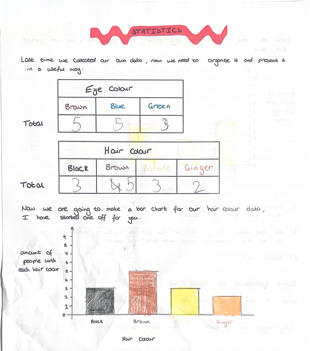
\includegraphics[scale = 0.4]{Images/Presenting_data.png}
            \caption{Example of bar chart created by a student}
        \end{figure}
    \end{columns}

\end{frame}

\begin{frame}{Session 5: Coordinate Grid}
    \begin{itemize}
        \item Deisgn:
        \begin{itemize}
            \item[-] Change mode of delivery
            \item[-] Make the session activite
            \item[-] Incorperating cooeprative groups in problem solving situations 
        \end{itemize}
        \item This session involved the students solving problems which would lead them from point to point on a coordinate grid
        \item The mathematics required was taken from lessons I had seen the students complete
        \item Each student had to solve one clue to lead them to the final anwer
        \item Evalutaion:
        \begin{itemize}
            \item[-] Students were very eager to solve clues
            \item[-] Students didn't understand coordinates as much as hoped
            \item[-] The problems given were effective reivison for the children - "We had to do really difficult maths that we learnt ages ago"
            \item[-] Sacrifised quantity of learning for enjoyment
        \end{itemize}
    \end{itemize}
\end{frame}


\begin{frame}{Session 6: 1-2 Nim}
    \begin{columns}
       \column{0.6\textwidth}
            \begin{itemize}
                \item Design:
                \begin{itemize}
                    \item[-] Student ownership, developing their own tool they can use in the future
                    \item[-] Students work together and share their solutions
                \end{itemize}
                \item This session involved the students developing their own strategies for a simple game
                \item This task generalises allowing students to learn some basic problem solving strategies

            \end{itemize}
        \column{0.4\textwidth}    
        \begin{figure}
            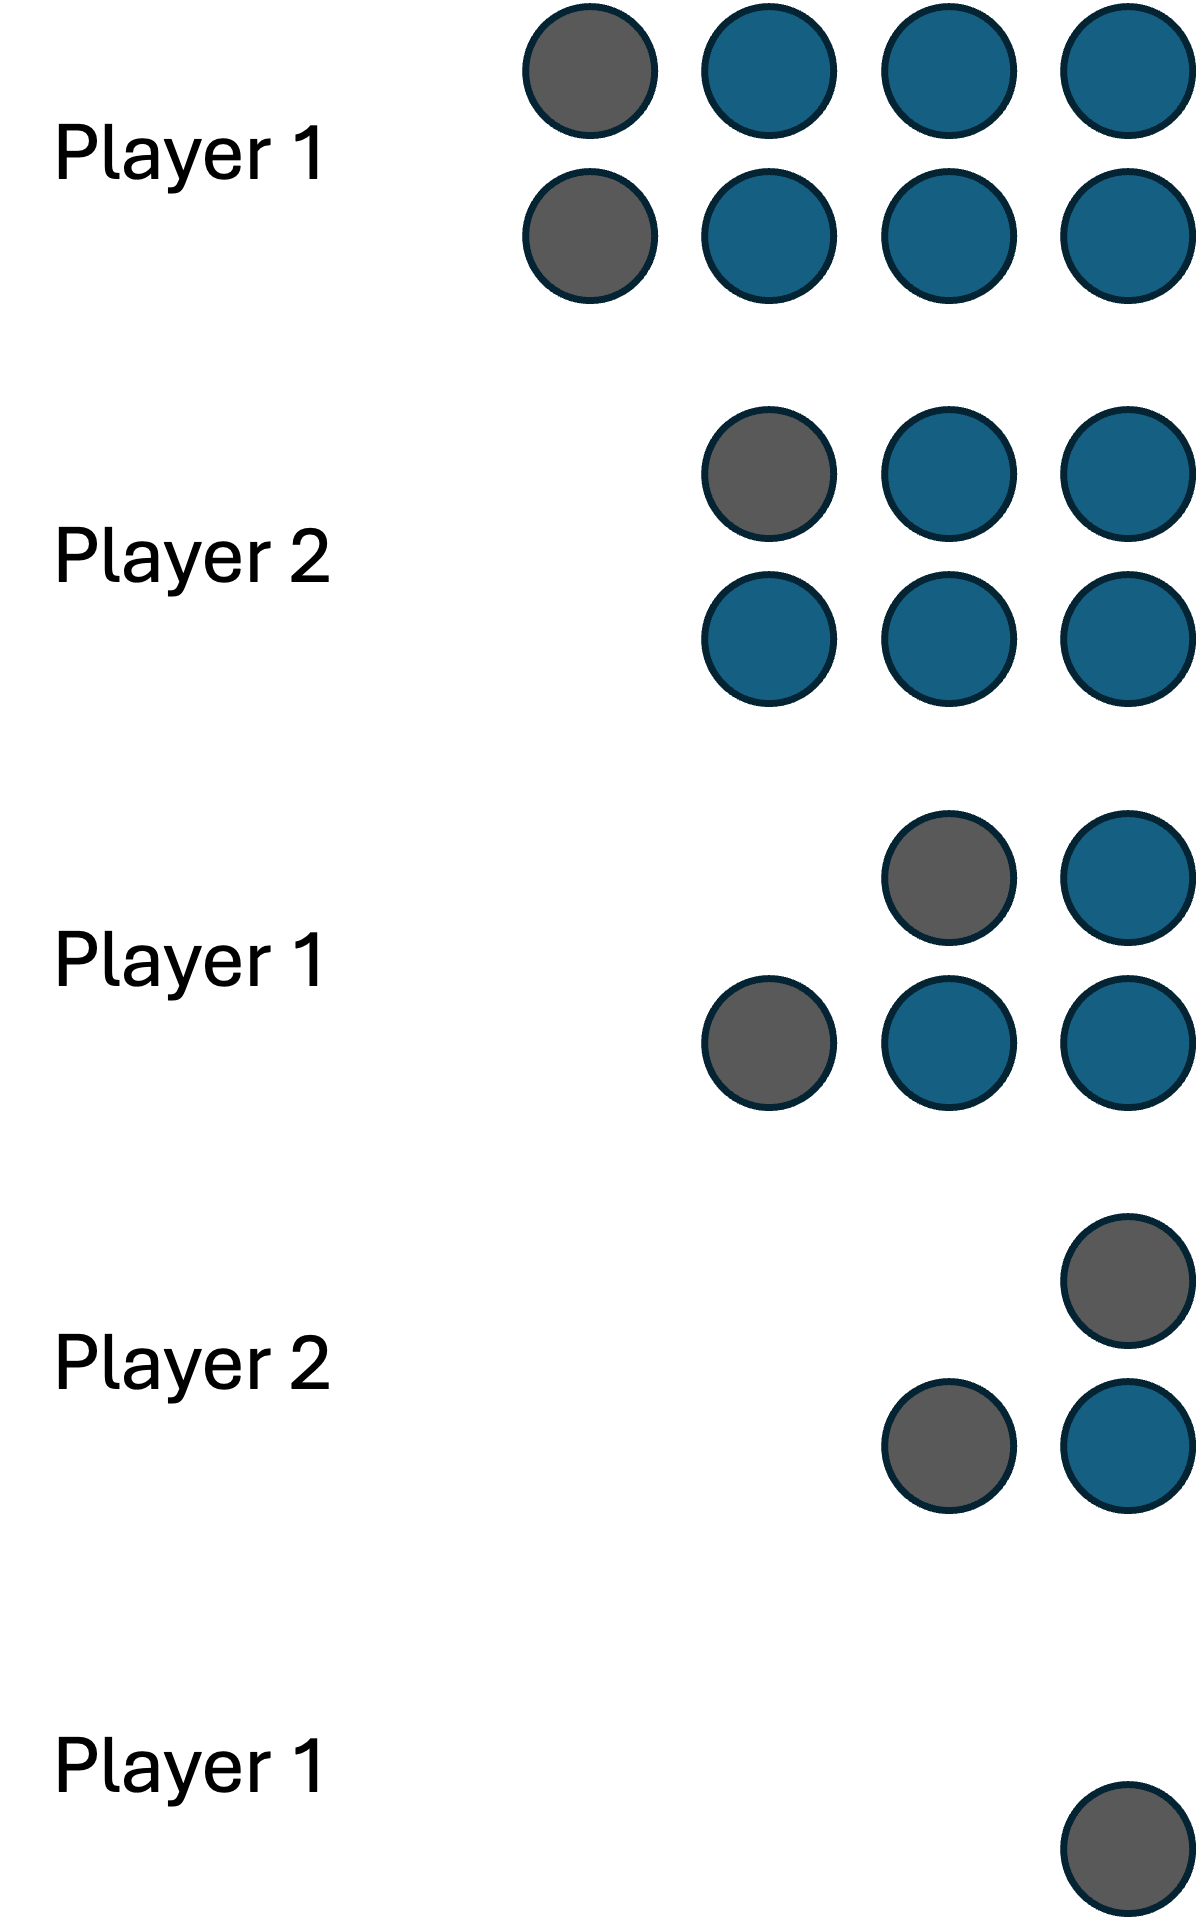
\includegraphics[scale = 0.45]{Images/1-2Nim_example.png}
            \caption{Example game of Nim}
        \end{figure}
    \end{columns}
\end{frame}

\begin{frame}{Session 6: 1-2 Nim}
    \begin{figure}
        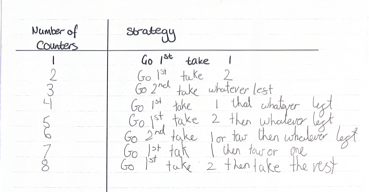
\includegraphics[scale = 0.6]{Images/1-2Nim.png}
        \caption{Example of data a student collected}
    \end{figure} 
            \begin{itemize}
                \item Evaluation:
                \begin{itemize}
                    \item[-] Students were keen to complete the task as they wanted to beat me
                    \item[-] Some of the more uninterested students seemed to benefit from this type of session
                \end{itemize}
            \end{itemize}

\end{frame}

\begin{frame}{Evaluation}
    \begin{itemize}
        \item Increasing maths confidence
        \begin{itemize}
            \item[-] Noticiable increase in participation throughout sessions
            \item[-] Difficult to distinguish causes of confidence
        \end{itemize}
        \item Decreasing maths anxiety
        \begin{itemize}
            \item[-] Design of sessions reduced maths anxiety within sessions
            \item[-] All students are willing to volunteer answers in sessions, which they may not do in regular maths lessons
            \item[-] Maths anxiety was definitely still present in some cases 
            \item[-] Many methods for dealing with maths anxiety are without of the scope of this project
        \end{itemize}
    \end{itemize}


\end{frame}

\end{document}